\chapter{Stream Ciphers}

\section{The problem with Vernam cipher}

There are few issues: generating a truly random key as long as the message, find a secure channel for transportation of the key to the message recipient and do this for every single message to be exchanged. In summary, the problem becomes to securely transfer large quantities of secure keys. There are two approaches that are seen as an improvement to Vernam cipher: stream ciphers and block ciphers.


\section{Symmetric encryption}
In stream ciphers we take a seed (a small vector of a few random bits) that must be kept secret, then build a keystream (a very long sequence of pseudorandom bits), finally xor the keystream with the plaintext bitwise to calculate the ciphertext. The problems are how are we going to generate a perfectly random keys of arbitrary size and how can we replicate the random streams of bytes for decryption.
In block ciphers we use the same key multiple times in a way that does not compromise the cipher. The problems are how can we reuse multiple times the same key without enabling an attacker to perform cipher-text only attacks and how can we avoid attackers to exploit the block structure.

These two ciphers are known as symmetric encryption algorithms, where stream ciphers perform operations in a way such that the plaintext is processed one bit at a time, and the algorithm selects one bit of plaintext, performs a series of operations on it, and then outputs one bit of ciphertext, block ciphers perform operations in a way such that the plaintext is processed in blocks (groups) of bits at a time, and the algorithm selects a block of plaintext bits (typically 64 bits), performs a series of operations on them, and then outputs a block of ciphertext bits.
Notice that a stream cipher can be seen as a block cipher with blocksize set to 1 bit, but there are also stream ciphers that process data in bytes, and hence could be regarded as block ciphers with a block size of 8, as a rule of thumb if the blocksize is less than 64 bits we talk about stream ciphers otherwise we talk about block ciphers.



\subsection{Stream ciphers}
The real work in designing a good stream cipher goes into designing the keystream generator. Keystream generators produce output which appears to be randomly generated, but is actually not randomly generated, these are referred to as pseudorandom generators. In many cases, stream ciphers combine the keystream with the plaintext in more complex ways than a simple bitwise xor operation.

\begin{figure}
	\centering
	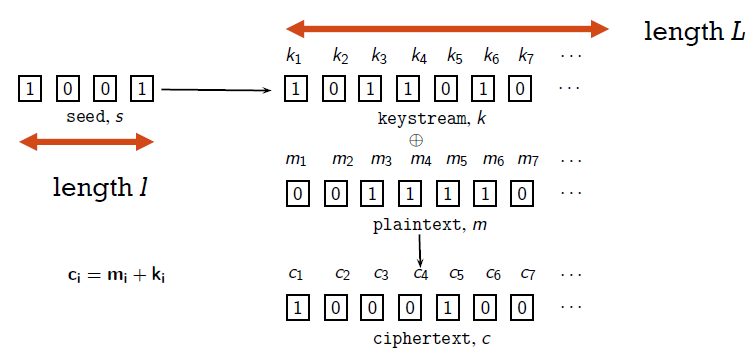
\includegraphics[width=0.7\linewidth]{Images/Chapter2/stream_ciphers}
	\caption{Stream cipher}
	\label{fig:stream_ciphers}
\end{figure}


For a stream cipher to be good, Eve should not be able to: recover the seed by making the set of possible seeds so large that and exhaustive search is very hard in practice and also predict the rest of the keystream by eliminating any patterns from the keystream.
More precisely: choose a short $l$-bit (much smaller than the lenght $L$ of the plaintext to be encrypted) seed $s$ as the encryption key and stretch the seed into a longer $L$-bit string (the key) that is used to mask the message and decrypt the ciphertext. The seed $s$ is stretched using some efficient, deterministic algorithm $G$ that maps $l$-bit strings (seeds) to $L$-bit strings(keys) \ref{fig:stream_ciphers}. Formally:
\begin{itemize}
	\item Encryption: $G(s) \oplus m$ for any seed $s$ (of size $l$) and plaintext $m$ (of size $L$)
	\item Decryption: $G(s) \oplus c$ for any seed $s$ (of size $l$) and ciphertext $c$ (of size $L$) where $G$ is called a pseudo-random number generator
\end{itemize}

Notice that if $l<L$, then by Shannon’s Theorem, stream ciphers cannot be perfect, however, if $G$ has certain properties, then stream ciphers are secure in practice. Suppose $s$ is a random $l$-bit string and $r$ is a random $L$-bit string, if Eve cannot effectively tell the difference between $G(s)$ and $r$, then it should not be able to tell the difference between stream ciphers and one-time pad. Since the one-time pad cipher is secure, so should be the stream cipher.

An algorithm that is used to distinguish a pseudo-random string $G(s)$ from a truly random string $r$ is called a statistical test. How might one go about designing an effective statistical test? One basic approach is the following: given an $L$-bit string, calculate some statistic, and then see if this statistic differs greatly from what one would expect if the string were truly random.
For example, a very simple statistic that is easy to compute is the number $k$ of $1$'s appearing in the string. For a truly random string, we would expect $k \approx L/2$. If the PRG $G$ had some bias towards either $0$-bits or $1$-bits, we could effectively detect this with a statistical test that, say, outputs 1 if $|k - 0.5L| < 0.01L$, and otherwise outputs 0. This statistical test would be quite effective if the PRG $G$ did indeed have some significant bias towards either $0$ or $1$.

A stream-cipher is well equipped to encrypt a single message from Alice to Bob. If two messages are encrypted with the same key there may be problems. As an example consider the case in which Alice and Bob want to exchange messages $m_1$ and $m_2$, let $c_1 = m_1 \oplus G(s)$ and $c_2 = m_2 \oplus G(s)$. If Eve is able to intercept both ciphertexts, then it is able to calculate $c_1 \oplus c_2 = ( m_1 \oplus G(s)) \oplus (m_2 \oplus G(s)) = (m_1 \oplus m_2) \oplus (G(s) \oplus G(s)) = m_1 \oplus m_2$, and as english text contains enough redundancy that given $m_1 \oplus m_2$, Eve can recover both $m_1$ and $m_2$ in the clear by using frequency analysis (given that both are sufficiently long). For this reason a stream cipher key should never be used to encrypt more than one message.

Stream-ciphers are said to be malleable since an attacker can cause predictable changes to the plaintext, this is because and attacker can intercept ciphertext $c$ and forwarding $c'=c \oplus d$, effectively the receiver will get $m' = c' \oplus G(s)= (c \oplus d) \oplus G(s) = (c \oplus G(s)) \oplus d = m \oplus d$. So again stream-ciphers do not provide integrity.
Regarding key management, stream ciphers do not require the key to be as long at the message encrypted, like the one time pad does. The key used to generate the keystream (and that must be distributed) is much shorter. In one-time pad the key has to be truly randomly generated, which involves costly generation techniques. The keystream in a stream cipher is pseudorandom and thus is much cheaper to generate. A keystream generator is a deterministic process since every time the same seed is input into the keystream generator, it will result in the same keystream being output. If we reuse a seed to produce the same keystream and then encrypt two plaintexts using the same portion of the keystream, then, just as in a one-time pad, the xor between the two ciphertexts will tell us the difference between the two corresponding plaintexts. We can avoid this problem by, e.g., making the keystream dependent on time varying data or generating the ciphertext with more complex operations than a xor.

In summary stream-ciphers do not give rise to error propagation as each bit in the ciphertext depends on just one bit in the plaintext and 1 bit transmission errors will result in 1 bit error in the plaintext, also they are very fast making them ideal for real time applications (e.g. mobile communication services) and easy to implement in hardware and don't require large memory capabilities. Since stream ciphers process data bitwise, it is crucial that sender and receiver keep their keystreams in perfect synchronization and 1 bit data loss may have catastrophic consequences as decryptions are performed on the wrong bits after the receiver is out of sync of the sender and re-synchronization mechanisms must be put in place to avoid these problems.


\subsection{Vigenère cipher}

It can be seen as a variant of Vernam cipher whereby the key is a sequence of bits of fixed length. The key, and plaintext are a string of bytes, to encrypt: XOR each character in the plaintext with the next character of the key and wrap around in the key as needed.

Vigenere cipher can be attacked by first determining the key length and determining each byte of the key by using frequency analysis.


\section{Examples of symmetric ciphers}

\begin{figure}
	\centering
	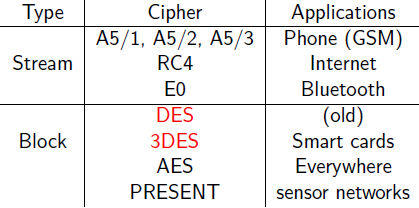
\includegraphics[width=0.4\linewidth]{Images/Chapter2/symmetric_encryption}
	\caption{Symmetric ciphers}
	\label{fig:symmetric_encryption}
\end{figure}

\subsection{Examples of stream ciphers}
\begin{itemize}
	\item RC4: Simple and fast stream cipher with a relatively low level of security, probably the most widely implemented stream cipher in software and widely used in SSL/TLS, WEP, and Microsoft Office
	\item A5/1: One of the stream cipher algorithms used in GSM to secure the communication channel over the air from a mobile phone to the nearest base station
	\item E0: The stream cipher algorithm used to encrypt Bluetooth communications
\end{itemize}

\section{Implementation of stream ciphers}

First we want to tackle the problem of generating a randomly a key (known as keystream) that is as long as possible. Keystream generators should be fast (as in computable in polynomial time as function of number $l$ of bits in the seed) and be secure, so intuitively, a string of $L$ bits produced by a keystream generator should look random. (i.e. it should be impossible in a polynomial amount of time in $l$ to distinguish between a truly random bit string of length $L$ and a string of the same length returned by the keystream generator). More importantly, a keystream generator, given the same seed it should produce the same sequence! The main components are \ref{fig:lfsr_internals}:
\begin{itemize}
	\item States: vector of bits organized in registers ($S_0,S_1,\cdots$)
	\item Update function: function mapping a state to the next state (clock function)
	\item Output function: function extracting a bit from a state. Concatenating all bits returned by this function, it is possible to obtain the keystream
	\item Key loading: function that takes the seed (secret) and a (public) initialization vector (IV) to compute the initial state for the update function. Each IV should be used only once.
\end{itemize}

\begin{figure}
	\centering
	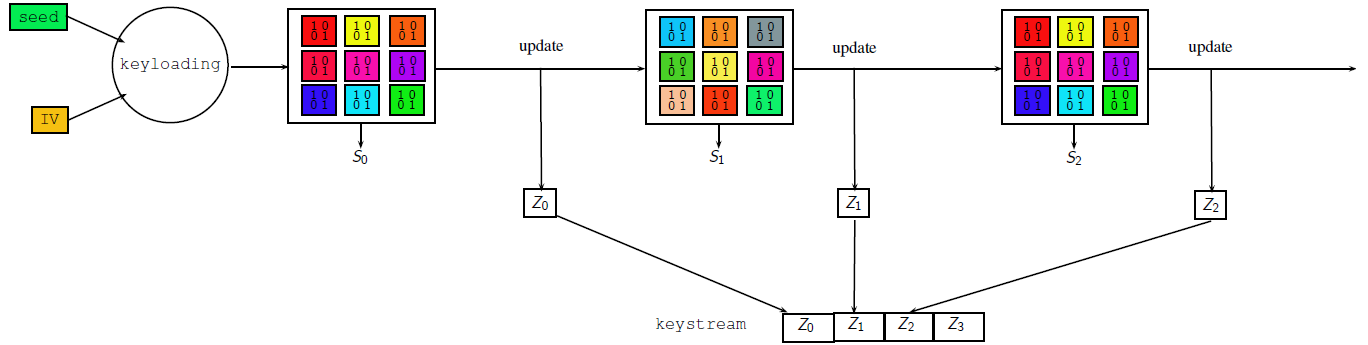
\includegraphics[width=0.9\linewidth]{Images/Chapter2/lfsr_internals}
	\caption{Stream ciphers internals}
	\label{fig:lfsr_internals}
\end{figure}

\section{Warm Up}

The first output bits strongly depend on the initial state. To avoid potential problems, it is customary to run a warm-up phase before starting encryption. This preliminary phase consists in applying the update function several times without outputting any bits of keystream and it is a highly recommended security best practice.
Given any initial state, the states are periodic, since they are in a finite number and at some point we will obtain again one of the previous states. The keystream is also periodic and this is impossible to avoid. The smallest number $i$ such that $update(\cdots(update(S)))=S$ is called the period of the keystream (it depends on the initial state), and as a requirement is that the period of the keystream shall be quite large, regardless of the initial state, and can be achieved by a suitable design of the update function.
As an example let's take an un update function as follows $f: (x,y,z) \Rightarrow (y+z,x,y)$. One can see that the repeated application of $f$ to the inital state $(1,0,1)$ will yield $(1,0,1) \Rightarrow (1,1,0) \Rightarrow (1,1,1) \Rightarrow (0,1,1) \Rightarrow (0,0,1) \Rightarrow (1,0,0) \Rightarrow (0,1,0) \Rightarrow (1,0,1)$ with a period of 7.
We are using linear functions because they are easy to implement and compute. Later we will see that linear functions (alone) should never be used.

\section{Linear feedback shift register (LFSR)}

A linear feedback shift register of length $n$ is a shift register composed by $n$ bits.
At any clock the following operations are executed:
\begin{itemize}
	\item the last bit on the right is output and forms part of the keystream
	\item the other bits in the register are shifted to the right by one position
	\item the XOR of some bits of the register are put in the first position on the left.
\end{itemize}

A shift register is a type of digital circuit using a cascade of flip flops (device which stores a single bit of data) where the output of one flip-flop is connected to the input of the next. Flip-flops share a single clock signal, which causes the data stored in the system to shift from one location to the next. 
A linear-feedback shift register (LFSR) \ref{fig:lfsr} is a shift register whose input bit is a linear function of its previous state. The most commonly used linear function of single bits is xor. An LFSR is usually a shift register whose input bit is driven by the xor of some bits of the overall shift register value, and the initial value of the LFSR is called the seed. Since the operation of the register is deterministic, the stream of values produced by the register is completely determined by its current (or previous) state.

\begin{figure}
	\centering
	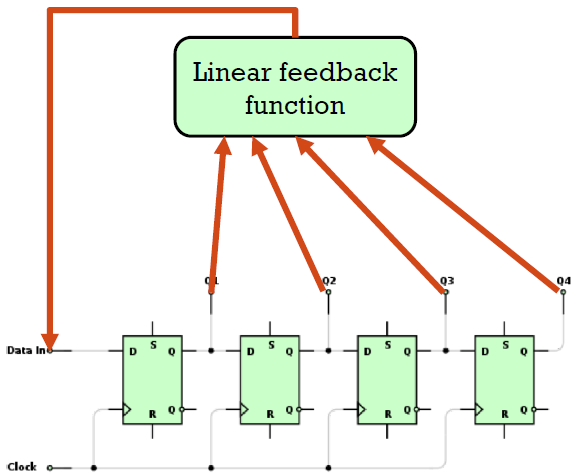
\includegraphics[width=0.7\linewidth]{Images/Chapter2/lfsr}
	\caption{Linear feedback shift register}
	\label{fig:lfsr}
\end{figure}

Since the register has a finite number of possible states ($2^n - 1$), it must eventually cycle. An LFSR with a well-chosen feedback
function can produce a sequence of bits that appears random and has a very long cycle. Typically the linear feedback function has the following form: $c_1 q_1 \oplus c_2 q_2 \oplus \cdots \oplus c_n q_n$ where $\oplus$ denotes the XOR operation. The non null $c_i$ are called taps.
Given a seed $s$, the period of $s$ is the number of steps the LFSR takes to return to $s$. The period of the LFSR is the maximum period achieved for any seed. For any number $n$ of taps there exists a maximal LFSR. Of the $2^{n}-1$ possible LFSRs, which taps correspond to maximal LFSRs? To answer this question we can use finite fields.

\section{LFSR and finite fields} 

Note: This is an informal introduction aiming to convey ideas with no attempt to mathematical rigour.

Consider addition modulo a certain number $N$, this is an instance of the notion of group, namely:
\begin{itemize}
	\item a set closed under a binary operation (addition modulo $N$)
	\item the operation is associative (addition modulo $N$ is so)
	\item there is an identity (0)
	\item each element has an inverse (e.g., 1 is the inverse of 11 when considering addition modulo N=12 as adding them gives 0)
\end{itemize}

The order of a group is the number of elements in its set (in the case of addition modulo a number $N$, the order of the group is $N$). The order of an element $a$ in a group is the number of times one needs to apply the operation to $a$ to produce the identity (example, the element 4 in the group modulo 12 has order 3 since $4+4+4=0$).
Consider now the multiplication modulo some number $N$. It is interesting to consider the order of its various elements that may be regarded to form cycles, containing the elements obtained by repeatedly applying the operation to the initial element up to its order, covering all (in case the order of the element is $N$) or some of the $N$ elements:
\begin{itemize}
		\item $3$ has order $3$ since $3*3 \bmod 13 = 9$, $9*3 \bmod 13 = 1$ and $1*3 \bmod 13 = 3$, the cycle generated is $\{ 3, 9, 1 \}$
	\item $2$ has order $12$ since $2*2 \bmod 13 = 4$, $4*2 \bmod 13 = 8$, $8*2 \bmod 13 = 3$, $3*2 \bmod 13 = 6$, and so on, the cycle generated is $\{ 2, 4, 8, 3, 6, 12, 11, 9, 5, 10, 7, 1 \}$
\end{itemize}

It is not difficult to see that there are other elements that can generate cycles containing all $12$ elements of the group, namely $6$, $7$, and $11$. Elements whose order is equal to the order of the group are called generators.
Multiplication modulo a prime number forms a group with similar properties to those discussed considering multiplication modulo 13. The order of an element is always a divisor of the group order by Lagrange's theorem. Because some elements are generators of the group itself, it is called a cyclic group. The number of generators of the "group multiplication modulo a prime number" $p$ having the full order $p - 1$, is $\varphi(p-1)$ where $\varphi(\cdot)$ is Euler's totient function, namely:
\[\varphi(n) = n \prod_{p|n}^{} (1- \frac{1}{p})\]

It counts the positive integers up to a given integer $n$ that are relatively prime to $n$. For $p=13$ in the previous example, we have that $\varphi(12) = 12 * \frac{1}{2} * \frac{2}{3} = 4$ which corresponds to what we have observed, i.e. that the 4 elements 2, 6, 7, and 11 are generators.

Consider again a generator $g=2$ of the group multiplication modulo the prime $p=13$. We can write $g^0$ to denote $1$, $g^1$ to denote $2$, $g^2$ to denote $4$, this allows us to list the elements of the group as powers of the generator, i.e. $1=g^0$, $2=g^1$, $4=g^2$, ... and this can be done for any group modulo a prime.

A ring is a group such that:
\begin{itemize}
	\item the group binary operation is commutative
	\item has another binary operation which is: closed over the ring's elements, associative, has an identity element and distributes over the group operation
\end{itemize}

A finite field has:
\begin{itemize}
	\item a finite set of elements
	\item two binary operations, which are abstract analogues to addition and multiplication
	\item analogues to subtraction and division using additive and multiplicative inverses
\end{itemize}

A \textbf{field} is a ring where both operations are commutative and have inverses. Intuitively a ring has addition, subtraction, and multiplication well-defined, a field adds division. A finite filed is also called Galois field and integer arithmetic modulo a prime is a finite field.

The simplest Galois field is $GF(2)$: it contains two elements (0 and 1) and the binary operations are addition and multiplication both modulo 2. On top of $GF(2)$ it is possible to construct: $GF(2)[x]$ that is the set of polynomials in x with only the elements of GF(2) allowed as coefficients and $GF(2)[x]/p$ that is the quotient of the set of polynomials by $p$.

Consider the polynomial $p(x)= x^4 + x +1$. In this case, $GF(2)[x]/p$ contains all possible polynomials of degree less than 4, namely \ref{fig:chapter2_screenshot006}

\begin{figure}
	\centering
	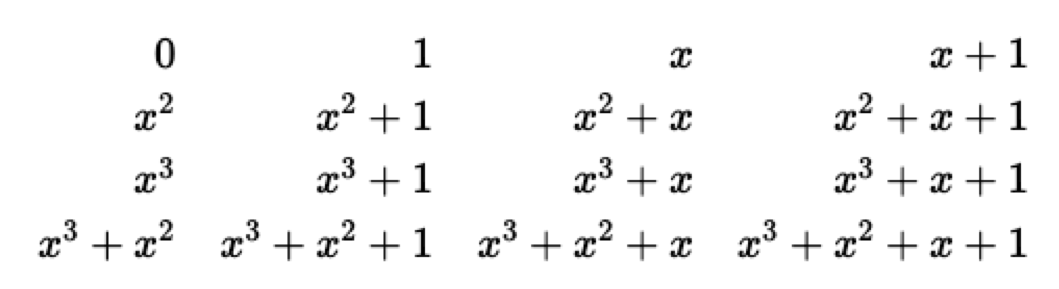
\includegraphics[width=0.7\linewidth]{Images/Chapter2/screenshot006}
	\caption{}
	\label{fig:chapter2_screenshot006}
\end{figure}
Polynomials $p(x)$ such that x is a generator of $GF(2)[x]/p(x)$ are called primitive polynomials.
In practice, this means that it is possible to start with 1 and, by using the procedure
below, it is possible to generate all the elements of $GF(2)[x]/p(x)$
\begin{itemize}
	\item consider $1$
	\item multiply by $x$ and if the result contains a term $x^N$ with $N$ = \emph{degree of} $p(x)$, then subtract $p(x)$
	\item stop when the result is $1$, this happens when the power of the generator is $2^N - 1$
\end{itemize}

Primitive polynomials $p(x)$ allow us to design maximal LFSRs by exploiting the following correspondence between these and $GF(2)[x]/p(x)$. In conclusion $GF(2)[x]/p(x)$ "corresponds" to $GF(2^N)$ when $p(x)$ is a primitive polynomial of degree $N$. These are useful because guarantee to generate the longest possible cycle.

\begin{figure}
	\centering
	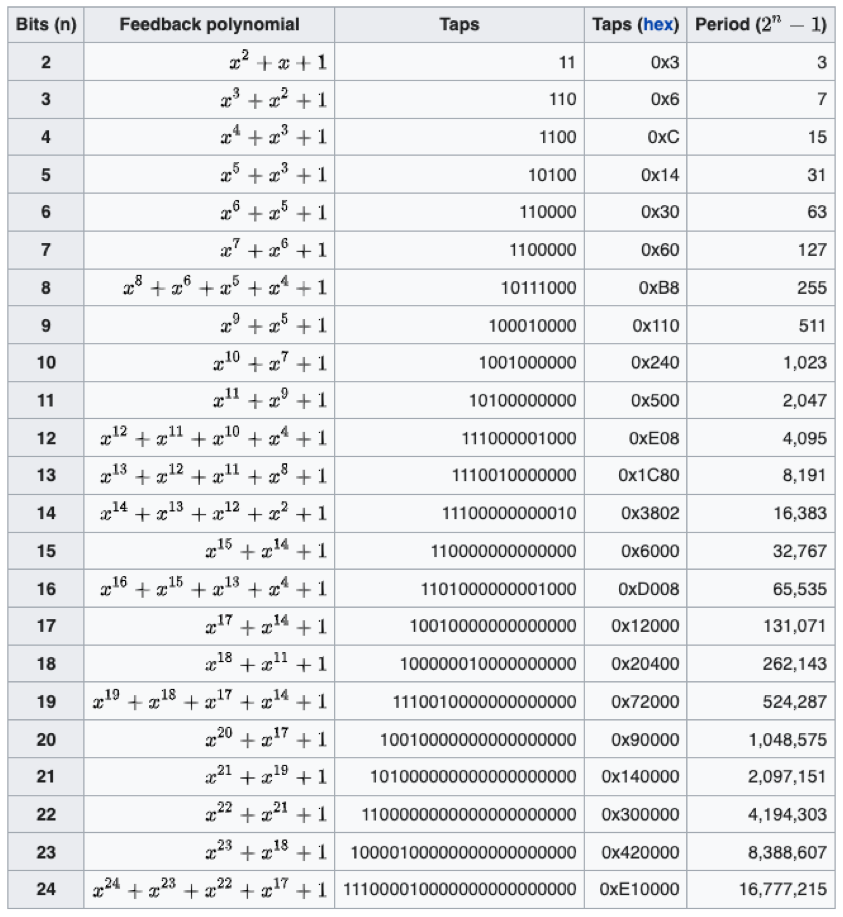
\includegraphics[width=0.7\linewidth]{Images/Chapter2/screenshot007}
	\caption{}
	\label{fig:chapter2_screenshot007}
\end{figure}

Given a maximum-length LFSR of n bits and reading $2^n - 1$ consecutive bits of the m-sequence that it produces, we have that:

\begin{itemize}
	\item one half of the bits are $1$ and one half are $0$ (actually the 1’s are one more than the 0’s)
	\item there are $2^{n-1}$ runs: $1/2$ of the runs has length $1$, $1/4$ of the runs has length 2, ..., $1/2^i$ of the runs has length $i$ (for $2 \le i \le n - 2$), there is only one run of $n-1$ zeros and none of the runs has $n-1$ ones, there is only one run of $n$ ones and none of the runs has $n$ zeros.
\end{itemize}

As an example consider using as feedback polynomial the primitive polynomial $x^5 + x^2 + 1$, hence the period is $2^5 - 1 = 31$ bits and we expect $2^{5-1} = 16$ runs. Starting from the state (10000), the obtained m-sequence is:
\[0000-1-00-1-0-11-00-11111-000-11-0-111-0-1-0-1\]

There are indeed 16 runs and 8 runs have length 1, 4 runs have length 2 , 2 runs have length 3, there is only 1 run of 4 zeros and none of 4 ones and there is only 1 run of 5 ones and none of 5 zeros.

\section{LFSR and linear algebra}

For analysing LFSRs, it is useful to investigate their relationships with Linear Algebra. For this, the key idea is the notion of companion matrix: given the polynomial $p(x) = c + c_1 * x + \cdots + c_n * n^n$ in $GF(2)[x]$ its companion matrix is:

\[
C(p) =
\left[ {\begin{array}{ccccc}
		0 & 0 & \cdots & 0 & c_{0}\\
		1 & 0 & \cdots & 0 & c_{1}\\
		0 & 1 & \cdots & 0 & c_{2}\\
		\vdots & \vdots & \ddots & \vdots & \vdots\\
		0 & 0 &\cdots & 1 & c_{n-1}\\
\end{array} } \right]
\]

It is possible to show that multiplication by $C$ is equivalent to multiplication by $x$ in $GF(2)[x]/p(x)$.
This connection allows us to consider the state recovery problem, i.e. predicting the state vector of the LFSR from its output bits. If we can solve this we can recover the initial state or, equivalently, the seed. And this requires polynomial time computations, this leads to the LFSRs main weaknesses: LFSRs can not be used directly in cryptography because of their linearity. Given any LFSR of length $n$, the $j$-th bit of the keystream, for can be obtained as a linear combination of its previous $n$ bits keystream.

Let the bits of the output sequence denoted by $a_0,\ldots,a_n$, there exists $n$ bits $\lambda_0,\ldots,\lambda_n$ such that $\sum_{i=0}^{n} \lambda_i a_i = 0, \lambda_n = 1$, note that the values $\lambda_0,\ldots,\lambda_n$ do not depend on when Eve starts intercepting the ciphertext.

Knowing the values of $\lambda_0,\ldots,\lambda_n$ is equivalent to knowing the feedback polynomial: $g=\sum_{i=0}^{n} \lambda_i x^i$ and thus being able to predict the keystream. Eve may obtain the required subsequence of the keystream mounting a known-plaintext or chosen-plaintext attack, hence LFSRs are vulnerable with respect to known-plaintext attacks and they must not be used as keystream generators, although they can be used as components in particular when iterated and combined by using some kind of non-linear functions. Linearity is good because it is easy to implement, but on the other hand is not secure enough.

\subsection{DVD encryption}
DVD encryption uses the CSS stream cipher to encrypt movie contents using a 40-bit secret key. The CSS stream cipher is particularly weak as it can be broken in far less time than an exhaustive search over all $2^{40}$ seeds \ref{fig:DVD}.

\begin{figure}
	\centering
	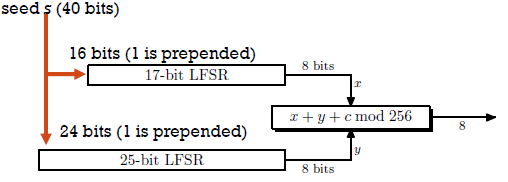
\includegraphics[width=0.7\linewidth]{Images/Chapter2/DVD}
	\caption{DVD CSS Encryption}
	\label{fig:DVD}
\end{figure}

The two LFSRs are run in parallel for 8 cycles and then the resulting bits are considered as integers and added modulo 256.
The simplest attack is simple bruteforce: suppose Eve knows the first 100 bytes of the output sequence, then just guess a 40 bits seed, run for 100 iterations and compare with the output sequence, if they match the seed was found, otherwise try another seed. And even smarter approach could be used to only attempt at most $2^{16}$ seeds.

\section{A5 family of ciphers}

\subsection{GSM}
The GSM (Global System for Mobile communication) standard was designed from 1982-1991, the level of security specifications regarding both authentication and encryption were limited: algorithms were never officially published (achieving security by obscurity), thus algorithms were reverse-engineered or leaked, leading to revelations of several possible attacks, and within a few months after the release, most of the cryptographic schemes had been compromised and some were even proven to be close to useless \ref{fig:GSM}.

\begin{figure}
	\centering
	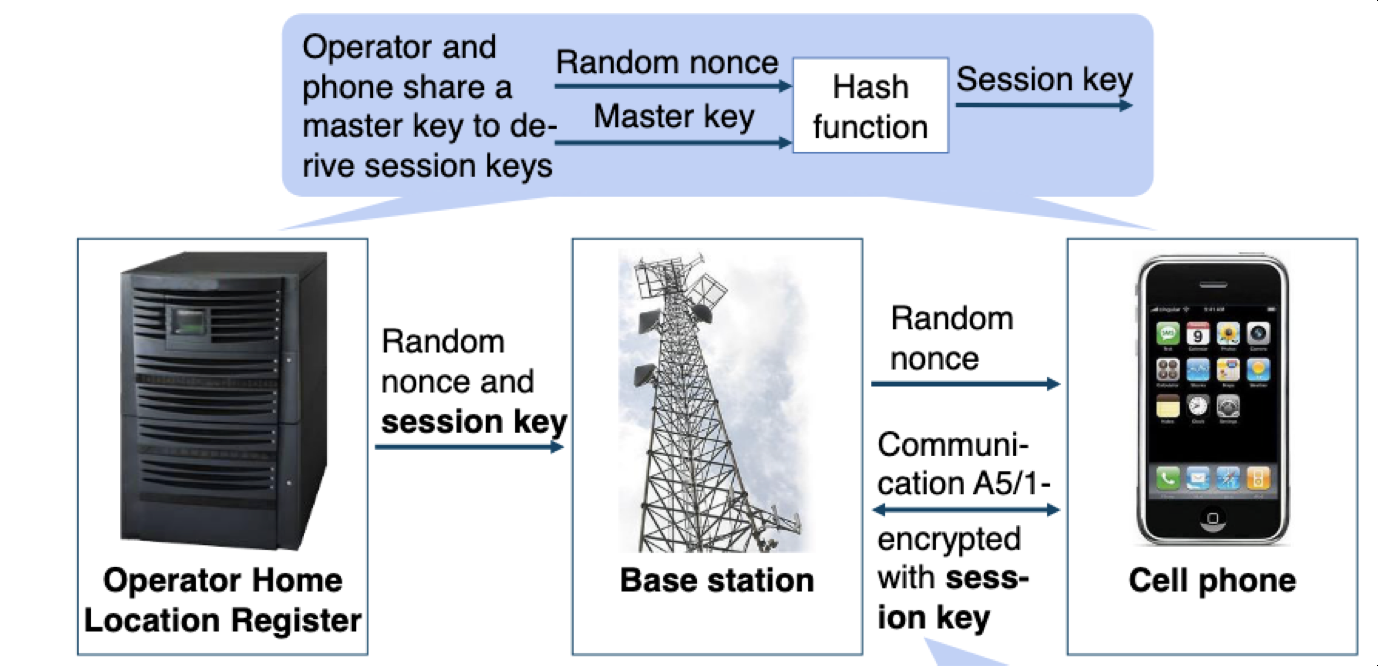
\includegraphics[width=0.7\linewidth]{Images/Chapter2/GSM}
	\caption{GSM}
	\label{fig:GSM}
\end{figure}

Each frame is numbered by a frame number, obtained by a frame counter initialized with 0 at conversation-start and incremented by $1 \bmod 2^{22}$ with each frame sent. An algorithm of the A5 family takes the session key $Kc$ (symmetric) and a frame counter $Fn$ and generates 228 pseudo random bits (PRAND) called a key stream. The keystream is then XORed with a 228 bit segment of plain text yielding 228 bits of ciphertext \ref{fig:A5ops}.

\begin{figure}
	\centering
	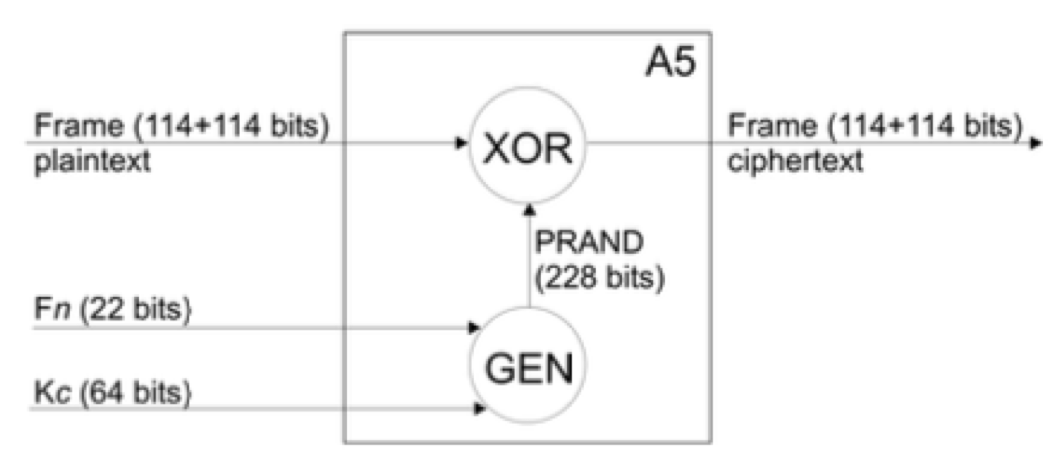
\includegraphics[width=0.7\linewidth]{Images/Chapter2/A5ops}
	\caption{A5 ciphers operation}
	\label{fig:A5ops}
\end{figure}


\subsection{A5/0}

It is the weakest of the A5 versions as it offers no encryption. It is a no-operation cipher, that generates the pseudo random bits by negating the input frame, thus leaving out the XOR function. The result is an algorithm that outputs the plain text it received as an input. This version is found in third world countries or countries with UN sanctions.

\subsection{A5/1}

It uses 3 LFSRs (with lenghts 19,22,23, total 64 bits of state) and has a keystream lenght of 228 bits \ref{fig:A51}.

\begin{figure}
	\centering
	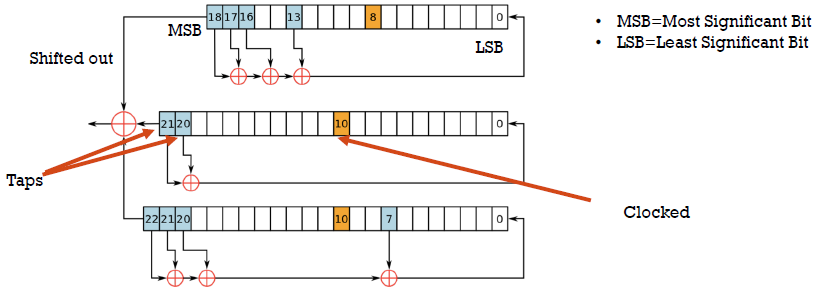
\includegraphics[width=0.7\linewidth]{Images/Chapter2/A51}
	\caption{A5/1}
	\label{fig:A51}
\end{figure}

When a register is clocked, its tapped bits are XORed and the result is stored in the registers LSB, the register MSB is shifted out of the register, and its value is forgotten.

In short first a seed (secret vector $K$ of 64 bits) is selected from the session key, then an initialization vector (public vector IV of 22 bits) that is the frame counter, from $K$ and $IV$ we get the inital state (namely a vector of 64 bits) using a keyloading function $kl(K,IV)$. The function $kl$ is defined by iteration: initially the registers contain all zeros, the bits in $K$ are injected by xor-ing them with other bits, and similarly for the bits of $IV$.
After the keyloading the warmup starts, the registers R1, R2, and R3 are irregularly clocked 100 times, without producing output, and it is as follows: in each step, the clock bits, each one among R1, R2, and R3 is updated if the clock bits agree with the majority of the clock bits. In this way, it is possible to show that each register clocks with a probability of $3/4$. At this point, the initialization of the registers is complete and the stream cipher is ready to output the key-stream. 

The keystream is is composed of 228 bits that are obtained in 228 steps, at each clock tick the update function is defined as follows:
\begin{itemize}
	\item The register R1 is updated if its clock bit agrees with the majority of the others
	\item The register R2 is updated if its clock bit agrees with the majority of the others
	\item The register R3 is updated if its clock bit agrees with the majority of the others
\end{itemize}

The ouput function is defined as: the xor of the output of the three registers R1, R2, R3 is the output bit.
After 228 bits of output, the key-loading phase is executed again.

\subsection{A5/2}

The key stream length remains the same as A5/1 but the number of LFSRs is increased to 4 respectively with lengths 19,22,23,17 with a total 81 bits of state.

In short a seed (secret vector $K$ of 64 bits) is selected, and an initialization vector (public vector IV of 22 bits), from $K$ and $IV$ we get the inital state (namely a vector of 64 bits) using a keyloading function $kl(K,IV)$. $kl$ and warmup are defined similarly to A5/1.

At each clock tick the update function is defined as follows:
\begin{itemize}
	\item $R_1$ is updated if $R_4[6]$ = maj($R_4[6]$, $R_4[13]$, $R_4[9]$)
	\item $R_2$ is updated if $R_4[13]$ = maj($R_4[6]$, $R_4[13]$, $R_4[9]$)
	\item $R_3$ is updated if $R_4[9]$ = maj($R_4[6]$, $R_4[13]$, $R_4[9]$)	
\end{itemize}

For the output a majority function is applied as non-linear filtering function to each of the first three registers
After a month an attack was found that could break the cipher almost in real time with a known plaintext attack.

\subsection{A5/3}
A5/3 is the last stream cipher of the A5 family and provides users with a higher level of security than both A5/1 and A5/2. It is based on the block cipher KASUMI. The keyspace is 128 bits and the message space is 64 bits \ref{fig:A53}.

\begin{figure}
	\centering
	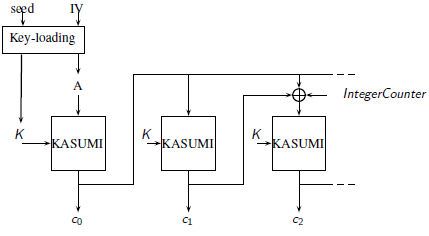
\includegraphics[width=0.7\linewidth]{Images/Chapter2/A53}
	\caption{}
	\label{fig:A53}
\end{figure}

The problem is that the key generated $Kc$ is only 64 bits, so the maximal exhaustive search complexity is (only) $2^{64}$. To make things worse $Kc$ generated only once after the cell phone registers with the network and stays active for all communication, until the telco requests a new one or the cell phone deregisters (so if one key is compromised every other communication is compromised until a new key is requested), and $Kc$ is artificially shortened in deployed systems when zeroing 10 bits, lowering search complexity to $2^{54}$, and encryption is applied after error correction.


\section{Remarks on the A5 Family}

\begin{itemize}
	\item A5/1 is affected by a number of serious weaknesses, and its use is strongly discouraged, since there are practical attacks that can break the cipher
	\item A5/2 is extremely weak and it can be broken in real time with inexpensive equipment; it is therefore no longer supported by new mobile phones
	\item A5/3 is the common standard for the new generation of mobile and it is considered secure, even though there do exist practical attacks to KASUMI that suggest some significant weaknesses of the cipher
\end{itemize}

\section{Practicality of attacking GSM communication}

In theory, the attacks are relatively simple. In practice, a considerable amount of hardware is necessary to actually intercept GSM communications. The hardware must at least consist of a radio receiver device which is capable of receiving and decoding digital data that is exchanged over-the-air. Hypothetically a simple GSM mobile phone already has all these capabilities (except the decrypting of an unknown A5 stream), so it might be possible to use such a phone for eavesdropping nevertheless a huge amount of know-how, time and money is needed.

\section{Bluetooth}
Bluetooth is a wireless technology standard invented by Ericsson in 1994 for exchanging data over short distances using short-wavelength UHF radio waves (Range: 2.4 to 2.485 GHz) from fixed and mobile devices.
The standard offers methods for generating keys, authenticating users, and encrypting data.
BLE was introduced in 2011 as Bluetooth 4.0, the main difference between BLE and Bluetooth is power consumption. BLE uses the AES cipher with 128-bit key length to provide data encryption and integrity over the wireless link.

\subsection{E0}

Used in Bluetooth standard and introduced in 1999. It uses 4 linear registers with lengths 25,31,33,39 with a total linear par of 128 bits. It has also one non linear register that is 4 bits. The update functions depend on the non-linear register \ref{fig:e0}.

\begin{figure}
	\centering
	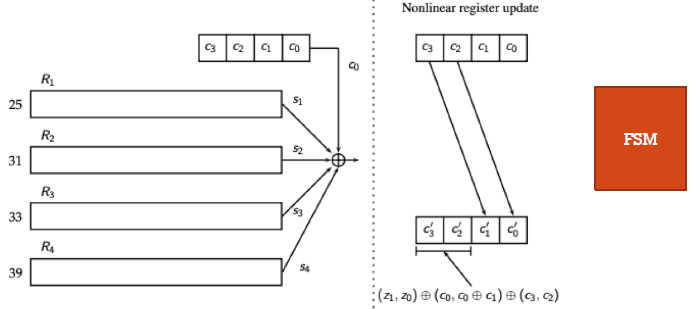
\includegraphics[width=0.7\linewidth]{Images/Chapter2/e0}
	\caption{}
	\label{fig:e0}
\end{figure}

\section{RC4}

Rivest Cipher 4 was designed in 1987. At first its implementation was trade secret, but then someone reverse engineered it, later Rivest confirmed that the code that was leaked was in fact correct. RC4 is used mainly because it is easy to implement in hardware and it is fast. RC4 was rapidly adopted in commonly used encryption protocols and standard like WEP and SSL.

RC4 generates a pseudorandom stream of bytes, the key stream. To generate the keystream, the cipher makes use of a secret internal state which consists of two parts: a permutation of all 256 possible bytes (denoted $S$) and two 8-bit index-pointers (denoted i and j). The permutation is initialized with a variable length key, typically between 40 and 2048 bits, using the so-called key-scheduling algorithm (KSA), once this has been completed, the stream of bits is generated using the pseudorandom generation algorithm (PRGA). While many stream ciphers are based on LFSRs (efficient in hardware but less so in software), the design of RC4 avoids the use of LFSRs and is ideal for software implementation, as it requires only byte manipulations.

The basic data structure needed is an array of 256 8-bit integers, called the state vector $S$ that is initialized with the encryption key $T$ with the following procedure:
\begin{enumerate}
	\item $S$ is initialized with entries from 0 to 255 in the ascending order
	\item $S$ is further initialized with the help of a temporary 256-element vector denoted T that also holds 256 integers. The vector T is initialized with the encryption key as follows: let $K$ be the encryption key represented as a vector 8-bit integers of size 16 (in case of a 128-bit key), i.e. K stores 16 non-negative integers whose values will be between 0 and 255, then initialize the 256-element vector T by placing in it as many repetitions of the key as necessary
	until T is full
	\item Use the 256-element vector T to produce the initial permutation of S as in \ref{fig:rc4_ksa}
\end{enumerate}

The keystream is generated with the algorithm in \ref{fig:rc4_keystream}
\begin{figure}
	\centering
	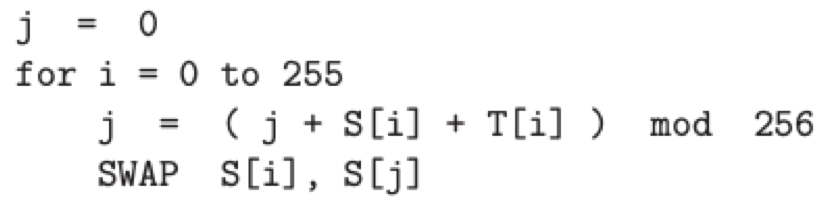
\includegraphics[width=0.7\linewidth]{Images/Chapter2/rc4_ksa}
	\caption{Key Scheduling Algorithm (KSA)}
	\label{fig:rc4_ksa}
\end{figure}

\begin{figure}
	\centering
	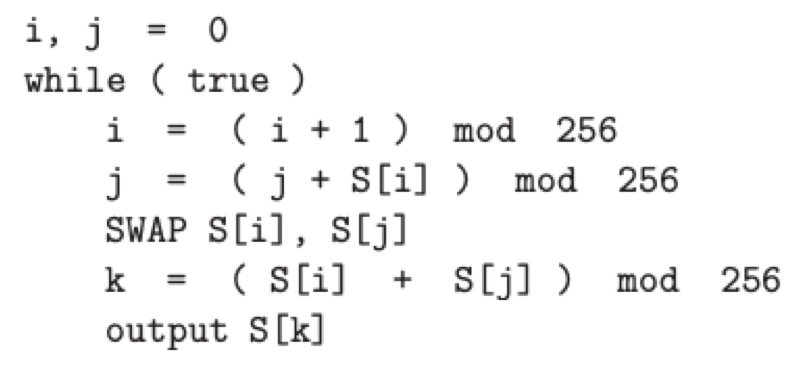
\includegraphics[width=0.7\linewidth]{Images/Chapter2/rc4_keystream}
	\caption{Generating the pseudorandom byte stream}
	\label{fig:rc4_keystream}
\end{figure}

But why use $j = (j + S[i] + T[i]) \bmod 256$? Because it works in practice. It is also easy to compute. But also the way you pick indexes is biased and this introduces vulnerabilities.

Theoretical analysis shows that for a 128 bit key length, the period of the pseudorandom sequence of bytes is likely to be greater than $10^{100}$, but it has been shown to be vulnerable to attacks especially if the beginning portion of the output pseudorandom byte stream is not discarded. As a consequence use of RC4 is prohibited in SSL/TLS protocol since 2015. 

WiFi security started with RC4 in the WEP protocol. After it was discovered that the encryption key used in WEP could be acquired by an adversary in almost no time, WiFi security has now moved on to the WPA2 protocol that uses AES for encryption.

Unlike modern stream ciphers, RC4 does not take a separate nonce alongside the key. If a single long-term key is to be used to securely encrypt multiple streams, the protocol must specify how to combine the nonce and the long-term key to generate the stream key for RC4. One approach to addressing this is to generate a "fresh" RC4 key by hashing a long-term key with a nonce. Unfortunately, many applications that use RC4 simply concatenate key and nonce; this gives rise to related key attacks that are famous for breaking the WEP standard.
Because RC4 is a stream cipher, it is more malleable than block ciphers. If not used together with other techniques (e.g., message authentication codes), then encryption is vulnerable to bit-flipping attacks.

Stream ciphers require a shared secret, a seed, which should be transmitted via a secure channel and once Alice and Bob have the seed, they can exchange via an insecure channel other parameters, like the IV and start encrypting/decrypting. The use of stream ciphers guarantees confidentiality. However, the stream cipher in itself does not guarantee that the seed has been exchanged securely, this has to be done in other ways. On the other hand, the attacker might tamper with the ciphertext and Alice/Bob will not understand immediately that the messages have been corrupted. In other words, stream ciphers provide neither authentication nor integrity.


\section{RC4 in WEP}

\subsection{WIFI Protocol}
\begin{itemize}
	\item Wired Equivalent Privacy (WEP) is the oldest protocol and has been proven to be vulnerable.
	\item Wi-Fi Protected Access (WPA) improved security but still vulnerable.
	\item Wi-Fi Protected Access II (WPA2) while not perfect is the most secure choice. It used two different types of cryptographic techniques to secure communication and those are Temporal Key Integrity Protocol (TKIP) and Advanced Encryption Standard (AES).
\end{itemize}

TKIP is used to authenticate the client and exchange messages in a secure way.
Authentication is based off the Pre Shared Key, a hard wired string written on the device.

\subsection{WIFI Authentication}

Client and the station have to agree on a key used to encrypt messages using symmetric encryption. How do we share this secret key? They have to agree over an insecure channel, so we need a protocol to do this. So the Client reads this preshared key on the device to authenticate to the device, but this key won't be used to encrypt messages! Because it is shared between clients! So TKIP used a key mixing function that takes as input this preshared key and an initialization vector and passing it to RC4 cipher initalization \ref{fig:rc4_wep}.

\begin{figure}
	\centering
	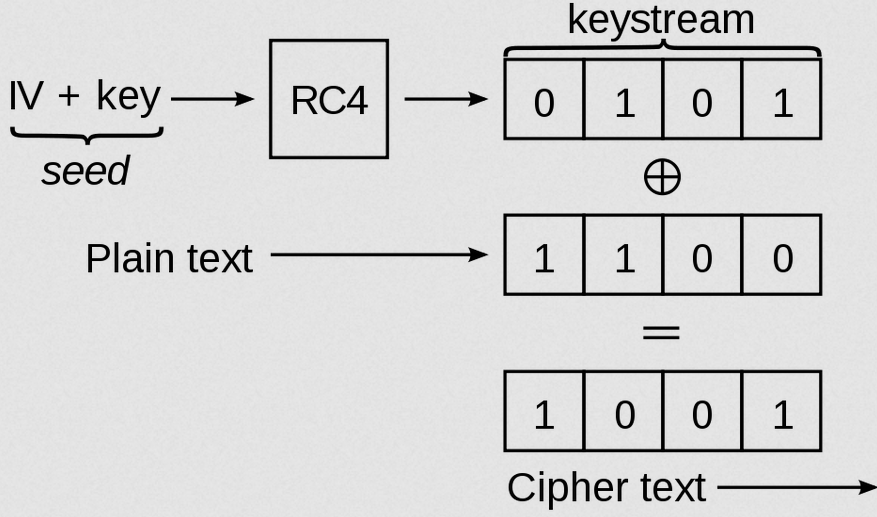
\includegraphics[width=0.7\linewidth]{Images/Chapter2/rc4_wep}
	\caption{}
	\label{fig:rc4_wep}
\end{figure}

\subsection{Security of WPA2}

Vulnerable to KRACK attack. It exploits a functionality where if a user is disconnected from WiFi then for reconnecting it performs an easier problem to derive a new session.